\paragraph{Sơ đồ tuần tự luồng xóa cuộc trò chuyện}

Luồng nghiệp vụ này mô tả
quá trình người dùng
thực hiện
xóa một cuộc trò chuyện,
đảm bảo tính nhất quán dữ liệu
giữa các dịch vụ
thông qua mẫu thiết kế Outbox Pattern
và giao tiếp qua RabbitMQ.

\subparagraph{Mô tả tổng quan}

\begin{itemize}

\item \textbf{Yêu cầu xóa cuộc trò chuyện:}
Người dùng
gửi yêu cầu
xóa cuộc trò chuyện
thông qua giao diện
bằng phương thức xóa.

\item \textbf{Đánh dấu xóa tạm thời:}
Dịch vụ trò chuyện
thực hiện một giao dịch CSDL
để đánh dấu xóa tạm thời cuộc trò chuyện
và lưu sự kiện xóa trò chuyện vào bảng sự kiện chờ gửi.

\item \textbf{Phản hồi nhanh:}
Dịch vụ trả về thông báo xóa thành công
cho giao diện ngay lập tức
để giảm thời gian chờ của người dùng.

\item \textbf{Chuyển tiếp sự kiện xóa:}
Tiến trình chuyển tin nhắn
quét bảng sự kiện chờ gửi định kỳ,
lấy ra các sự kiện
xóa cuộc trò chuyện
và gửi vào hàng đợi tin nhắn.
Sau khi gửi tin nhắn thành công,
tiến trình cập nhật trạng thái sự kiện
thành đã hoàn thành trong CSDL.

\item \textbf{Xử lý xóa ở dịch vụ chatbot:}
Dịch vụ chatbot
nhận sự kiện xóa
trò chuyện từ hàng đợi tin nhắn,
tiến hành đánh dấu xóa tạm thời cuộc trò chuyện tương ứng
theo định danh cuộc trò chuyện
và định danh người dùng trong CSDL chatbot,
sau đó gửi xác nhận hoàn thành xử lý.

\end{itemize}

\begin{figure}[H]
\centering
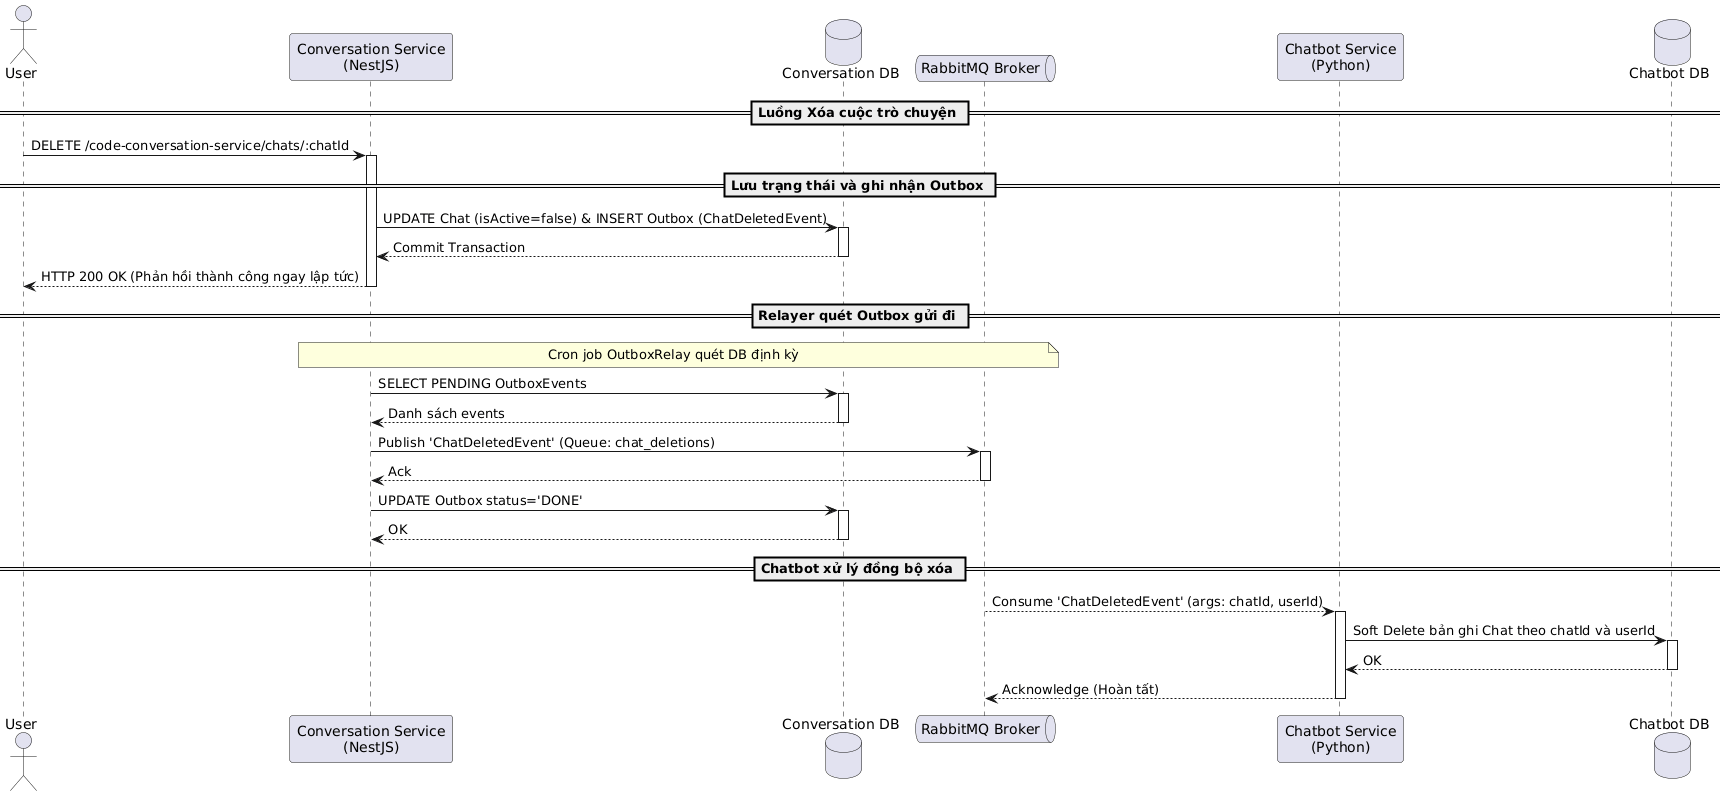
\includegraphics[width=0.95\textwidth]{contents/Sequence/UML-Sequence-UserDeleteChat.png}
\caption{Sơ đồ tuần tự luồng xóa cuộc trò chuyện}
\end{figure}

\begin{table}[H]
\centering
\renewcommand{\arraystretch}{1.3}

\begin{tabular}{|l|l|p{5cm}|}
\hline
\textbf{Thành phần} & \textbf{Phân loại} & \textbf{Vai trò trong hệ thống} \\ \hline
User & Actor & Người dùng thực hiện thao tác gửi yêu cầu để xóa một cuộc trò chuyện. \\ \hline
Conversation Service & Microservice & Dịch vụ trò chuyện tiếp nhận yêu cầu từ người dùng, cập nhật trạng thái xóa, ghi nhận sự kiện vào Outbox và dùng Cron job để relay sự kiện. \\ \hline
Conversation DB & Database & CSDL lưu trò chuyện và bảng Outbox. \\ \hline
RabbitMQ Broker & Message Broker & Message Broker nhận sự kiện và phân phối đến các dịch vụ theo dõi. \\ \hline
Chatbot Service & Microservice & Dịch vụ AI đóng vai trò tiêu thụ (Consumer), lắng nghe sự kiện xóa để đồng bộ hóa dữ liệu. \\ \hline
Chatbot DB & Database & CSDL lưu chi tiết các tin nhắn của cuộc trò chuyện. \\ \hline
\end{tabular}
\caption{Các thành phần tham gia luồng xóa cuộc trò chuyện}
\end{table}
